\chapter{Results}

In this section we will present and reitterate the constributions we have made as a result of this project.

We have contributed with a simplified Python version of the original GFN2-xTB Fortrain implementation. The implementation and validation of the dispersion term is not complete, and we have not implemented the self-consistent charges that is used to iteratively rerun the computations to improve the accuracy of the result. Despite missing these, we are surprised to have all the other terms when looking at the size of the codebase. This Python implementation should hopefully be make the xTB algorithm more approachable in terms of understanding and when it is ported to SYCL as a lockstep GPU implementation.

We have contributed with a reproducable testing framework, which should provide value to our successors.

We have contributed with a reproducable and easy way to build, run, and patch xtb, its dependencies, and even the challenging to run older GPU compatible version 6.4.0.

We have contributed with all of our learnings and knowledge about the xTB algorithm and its codebase.

We have contributed with ideas and insights that would make a massively lockstep implementation possible.
We have gone into depth about hardware requirements, why this approach is a good fit, and why it is better than regular task parralization. We have explained necessary considerations to make this approach possible and effective.
We have also transformed code snippets to give examples on how to make it adhere to requirements of a lockstep kernel, and how to optimize the code to our problem domain by only considering carbon atoms.

% TODO: ASMUS!!!! Skriv vores quantum contributions >w<
%In continuation of this, we have designed our own quantum circuits and proposed how to use the arithmetic operations they implement to further optimize the xTB algorithm with computational quantum algorithmic approaches.



\section{Validation}



\begin{figure}[H]
\centering
\begin{subfigure}{.5\textwidth}
  \centering
  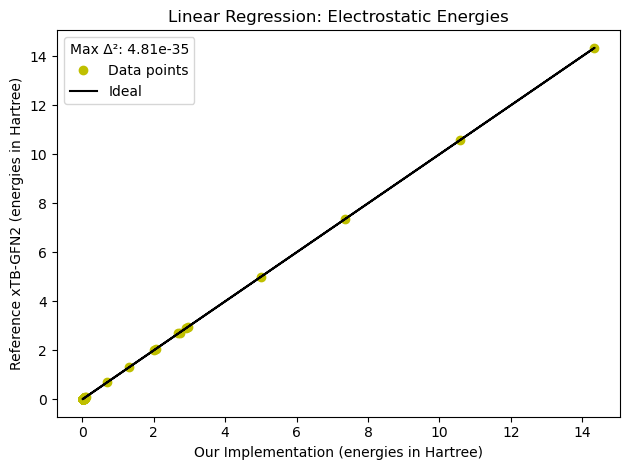
\includegraphics[width=.8\linewidth]{images/results/es_check}
  \caption{es check}
  \label{fig:es_check}
\end{subfigure}%
\begin{subfigure}{.5\textwidth}
  \centering
  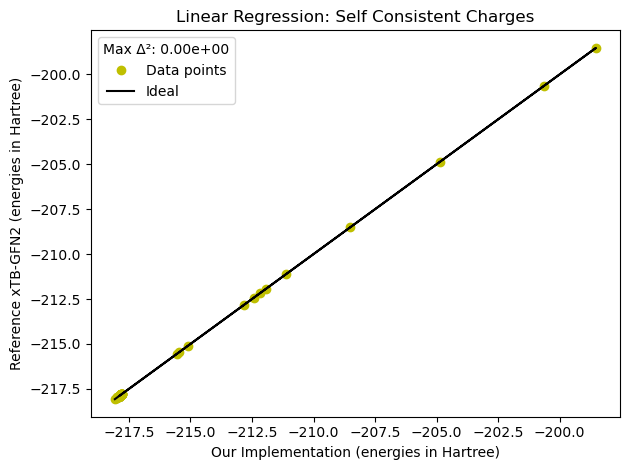
\includegraphics[width=.8\linewidth]{images/results/scc_check}
  \caption{scc check}
  \label{fig:scc_check}
\end{subfigure}
\end{figure}

\section{Benchmarks}
